\chapter{Metodologia}\label{ch:metodologia}
%  VISÃO GERAL DO CAPÍTULO
A metodologia caracteriza a distribuição espacial e a magnitude dos máximos de precipitação e vento associados aos ciclones extratropicais do Atlântico Sul, mediante um referencial centrado no sistema e condicionado pela fase do ciclo de vida e pela região de ciclogênese.
A estratégia segue cinco etapas: (1) definição das fontes de dados; (2) construção e estratificação das populações de ciclones; (3) processamento semilagrangeano dos campos de superfície; (4) caracterização estatística univariada mediante estimação de densidade e análise EOF; e (5) análise multivariada (MEOF) e construção de protótipos estruturais.
Os protótipos se organizam em $3 \times 4$ painéis (3 regiões de ciclogênese $\times$ 4 fases evolutivas) para a População Global (PG) e o subconjunto p90.

%  SEÇÃO M1 — DADOS
\section{Dados}\label{sec:datos}
\subsection{Reanálise ERA5}\label{sec:datos_era5}
Utiliza-se a reanálise de quinta geração do ECMWF, ERA5 \citep{hersbach2020era5}, mediante o conjunto de dados \textit{``ERA5 hourly data on single levels from 1940 to present''} \citep{hersbach_era5_2023b} para o período 1979--2020.
A resolução espacial ($\sim$31 km) e temporal (horária) do ERA5, juntamente com sua maior densidade de trajetórias e representação de estruturas de mesoescala em relação a reanálises anteriores \citep{gramcianinov2020analysis}, justificam sua escolha para o catálogo de trajetórias.
No entanto, \citet{chen2024evaluation} demonstram que o ERA5 subestima sistematicamente os extremos dos 5\% de ciclones extratropicais mais intensos, com vieses de $-10.2\%$ em vento e $-22.6\%$ em precipitação em relação a observações nos Estados Unidos da América.
Por isso, os resultados obtidos para p90 devem ser interpretados como estimativas conservadoras da intensidade real dos eventos.

\subsection{Variáveis meteorológicas}\label{subsec:variables}
A análise é realizada a partir de campos horários de ERA5, com as seguintes variáveis de superfície:

\begin{itemize}
    \item Precipitação total acumulada (\texttt{tp}, em mm\,h$^{-1}$).
    \item Magnitude do vento em superfície a 10 m (\texttt{wind10}, em m\,s$^{-1}$).
\end{itemize}

A escolha de ambas as variáveis responde à natureza morfológica dos ciclones extratropicais e à estrutura de seus campos de precipitação e vento, fundamentada na Seção~\ref{sec:tb_compound_def} dos Fundamentos.
Essa abordagem descreve a configuração espacial típica dos campos de superfície em cada fase evolutiva e permite avaliar a eventual co-ocorrência dos máximos de ambas as variáveis, como primeira aproximação à análise multivariada (MEOF) detalhada na Seção~\ref{subsec:eof_multivariado}.

\subsection{Base de trajetórias e fases}\label{sec:bd_ciclones}
Esta tese não realiza a detecção, o rastreamento nem a classificação de fases dos ciclones.
Emprega-se a base de trajetórias e fases desenvolvida em \citet{coutodesouza2024thesis}, construída sobre o catálogo de \citet{gramcianinov2020analysis} (Tabela~\ref{tab:tracking_params}) e com as fases classificadas mediante \textit{CycloPhaser} \citep{deSouza2025CycloPhaser}.
Essa classificação não distingue explicitamente os sistemas que, durante seu ciclo de vida, poderiam transicionar para uma estrutura subtropical (núcleo quente em altitude) no sentido de \citet{hart2003cyclone}; não se pode descartar que uma fração dos sistemas catalogados, particularmente em SBR e LPB, inclua casos em transição para essa estrutura.

\begin{table}[ht]
\centering
\caption[Parâmetros e filtros da base de trajetórias]{Parâmetros técnicos e filtros aplicados na base de dados de trajetórias \citep{gramcianinov2020analysis}.}
\label{tab:tracking_params}
\begin{tabular*}{\textwidth}{@{\extracolsep{\fill}}ll}
\hline
Parâmetro & Especificação \\
\hline
Fonte de dados & ERA5 (ECMWF) \\
Resolução espacial & $\sim$31 km ($0.25^\circ \times 0.25^\circ$) \\
Variável de rastreamento & Vorticidade relativa a 850 hPa ($\zeta_{850}$) \\
Duração mínima & 24 horas \\
Deslocamento mínimo & 1000 km \\
\hline
\end{tabular*}
\end{table}


A partir dessa base, selecionam-se os ciclones de estudo (Seção~\ref{sec:poblaciones_estudio}) e extraem-se os campos de ERA5 nos mesmos instantes de cada trajetória.
Os fundamentos físicos do uso de $\zeta_{850}$ e da segmentação em quatro fases são expostos nas Seções~\ref{subsec:tb_zeta} e~\ref{subsec:tb_fases} dos Fundamentos. A Tabela~\ref{tab:fases_def} resume essas fases.

\begin{table}[ht]
\centering
\caption[Definição das fases do ciclo de vida]{Definição das fases do ciclo de vida na base de dados utilizada \citep{coutodesouza2024new}.}
\label{tab:fases_def}
\begin{tabular*}{\textwidth}{@{\extracolsep{\fill}}lp{10cm}}
\hline
Fase & Descrição Dinâmica \\
\hline
Incipiente (Ic) & Etapa inicial de organização do vórtice, anterior à queda abrupta de pressão. \\
Intensificação (It) & Período de rápido crescimento da vorticidade ciclônica (taxa de variação negativa intensa). \\
Maturidade (M) & Etapa em que o sistema alcança sua intensidade máxima (pico de vorticidade) e estabilização relativa. \\
Decaimento (D) & Fase final de debilitamento progressivo do vórtice (ciclólise) e dissipação. \\
\hline
\end{tabular*}
\end{table}


%  SEÇÃO M2 — POPULAÇÕES DE ESTUDO

\section{Populações de estudo}\label{sec:poblaciones_estudio}

A base de trajetórias se divide em uma população de referência e, a partir dela, um subconjunto de alta intensidade ($p90$), como detalhado na Seção~\ref{subsec:tb_poblaciones}
Ambas as populações são construídas de forma independente para cada uma das três regiões de ciclogênese (SBR, LPB e ARG), delimitadas mediante domínios geográficos fixos baseados na taxonomia de \citet{gramcianinov2019properties} e detalhados na Tabela~\ref{tab:regiones_coords}.
Essa estratificação geográfica responde ao fato de que as regiões apresentam regimes dinâmicos diferenciados, discutidos na Seção~\ref{sec:tb_regiones}.

\begin{table}[ht]
\centering
\caption[Coordenadas dos domínios de ciclogênese]{Coordenadas geográficas dos domínios de ciclogênese definidos segundo \citet{gramcianinov2019properties}.}
\label{tab:regiones_coords}
\begin{tabular*}{\textwidth}{@{\extracolsep{\fill}}lll}
\hline
Região & Longitude & Latitude \\
\hline
Sul-Sudeste do Brasil (SBR) & $52^\circ\text{W} - 37^\circ\text{W}$ & $38^\circ\text{S} - 23^\circ\text{S}$ \\
La Plata/Uruguai (LPB) & $69^\circ\text{W} - 52^\circ\text{W}$ & $38^\circ\text{S} - 23^\circ\text{S}$ \\
Patagônia/Argentina (ARG) & $70^\circ\text{W} - 50^\circ\text{W}$ & $55^\circ\text{S} - 39^\circ\text{S}$ \\
\hline
\end{tabular*}
\end{table}


\subsection{População Global (PG): referência}\label{subsec:grupo_global}

A População Global estabelece o comportamento morfológico e estatístico médio dos ciclones com desenvolvimento típico e completo na região.
Aplica-se um critério de coerência evolutiva, selecionando unicamente os sistemas que cumpriram dois critérios simultâneos:

\begin{enumerate}
    \item Ciclo de vida completo: Presença confirmada e sequencial das quatro fases de desenvolvimento, incipiente (\textit{incipient}), intensificação (\textit{intensification}), maturidade (\textit{mature}) e decaimento (\textit{decay}).
    \item Ausência de fases complexas: Exclusão categórica de sistemas que desenvolveram fases secundárias, de reintensificação (p. ex., \textit{intensification~2}, \textit{mature~2}) ou fases residuais (\textit{residual}).
\end{enumerate}

Isso elimina o ruído de sistemas efêmeros ou de evolução errática.
Para cada ciclone da PG, identifica-se o valor mais negativo de vorticidade relativa a 850 hPa, $\zeta_{850}^{\min}$, alcançado em algum momento de sua vida, como métrica de intensidade para a extração posterior do subconjunto p90.

A Figura~\ref{fig:loc_vort_global} sintetiza a densidade de probabilidade da localização onde os ciclones da PG alcançam seu $\zeta_{850}^{\min}$ ao longo de seu ciclo de vida, com o número de ciclones detalhado na Tabela~\ref{tab:conteo_ciclones}.

\begin{figure}[htbp]
\centering
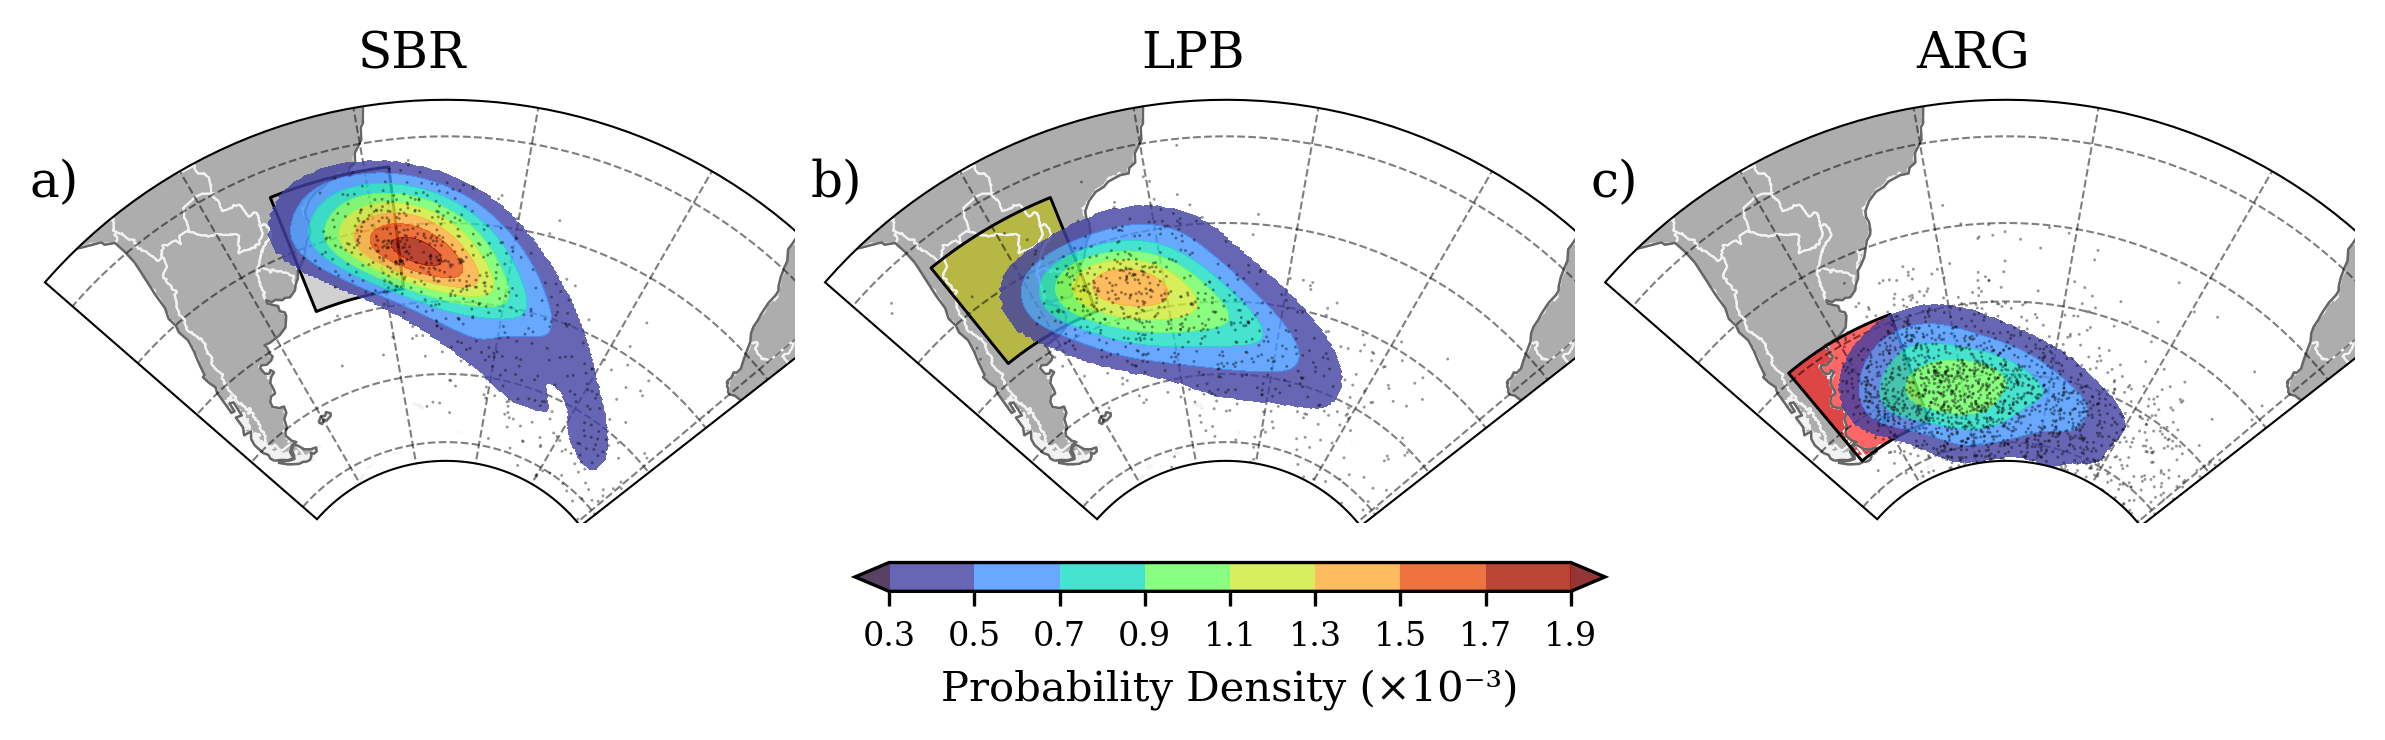
\includegraphics[width=\textwidth]{images/geral/vort_global_vf.png}
\caption[Localização do mínimo de vorticidade (População Global)]{Distribuição espacial da densidade de probabilidade da localização onde os ciclones da PG alcançam sua menor vorticidade relativa a 850~hPa ($\zeta_{850}^{\min}$) ao longo de seu ciclo de vida. a), b) e c) correspondem às regiões de ciclogênese SBR, LPB e ARG, respectivamente. Os contornos de cores indicam a densidade de probabilidade ($\times 10^{-3}$) e os pontos cinzas marcam as posições individuais dos mínimos.}
\label{fig:loc_vort_global}
\end{figure}


\subsection{Subconjunto de alta intensidade (p90)}\label{subsec:subconjuntos_intensidad}

Para avaliar os padrões espaciais em função da severidade dinâmica do sistema, extrai-se da PG, de forma independente para cada região de ciclogênese, os 10\% de ciclones com os valores mais negativos de $\zeta_{850}^{\min}$ (um decil da distribuição), obtendo o subconjunto $p90$ (detalhado em \ref{subsec:tb_poblaciones}).

A Tabela~\ref{tab:conteo_ciclones} documenta a redução do tamanho amostral desde a base bruta até a PG e o subconjunto p90.

\begin{table}[htbp]
\centering
\caption[Número de ciclones selecionados por região]{Número de ciclones selecionados por região. A coluna ``Total'' refere-se à base de trajetórias bruta e ``População Global'' aos sistemas com um ciclo de vida completo. A coluna ``Subconjunto'' indica o tamanho amostral para o subconjunto analisado (p90), equivalente a 10\% da População Global.}
\label{tab:conteo_ciclones}
\begin{tabular*}{\textwidth}{@{\extracolsep{\fill}}lccc}
\hline
Região & Total & População Global & Subconjunto \\
\hline
ARG & 4015 & 1980 & 198 \\
SBR & 1486 & 641  & 64  \\
LPB & 1288 & 669  & 67  \\
\hline
\end{tabular*}
\end{table}


A análise da fase em que se registra o pico de vorticidade (Tabela~\ref{tab:fase_max_intensidad}) mostra que p90 respeita a estrutura dinâmica dominante. Cerca de 83\% dos casos alcança sua intensidade máxima ($\zeta_{850}^{\min}$) durante a fase de maturidade, frente a menos de 5\% durante o decaimento.

\begin{table}[htbp]
\centering
\caption[Fase evolutiva de máxima intensidade dinâmica]{Distribuição percentual da fase evolutiva em que se registra a máxima intensidade dinâmica ($\zeta_{850}^{min}$), calculada como média entre as três regiões de ciclogênese.}
\label{tab:fase_max_intensidad}
\begin{tabular*}{\textwidth}{@{\extracolsep{\fill}}lcccc}
\hline
\textbf{Fase} & \textbf{População Global (\%)} & \textbf{p90 (\%)} \\
\hline
Incipiente       & $\sim$0.1 & ---  \\
Intensificação  & 13.2      & 11.7 \\
Maturidade       & 71.8      & 83.4 \\
Decaimento      & 14.9      & 4.9  \\
\hline
\end{tabular*}
\end{table}


A Figura~\ref{fig:loc_vort_p90} mostra a distribuição espacial da densidade de probabilidade da localização do mínimo de vorticidade do subconjunto p90.

% Figura para o subconjunto p90 (Subseção 2)
\begin{figure}[htbp]
\centering
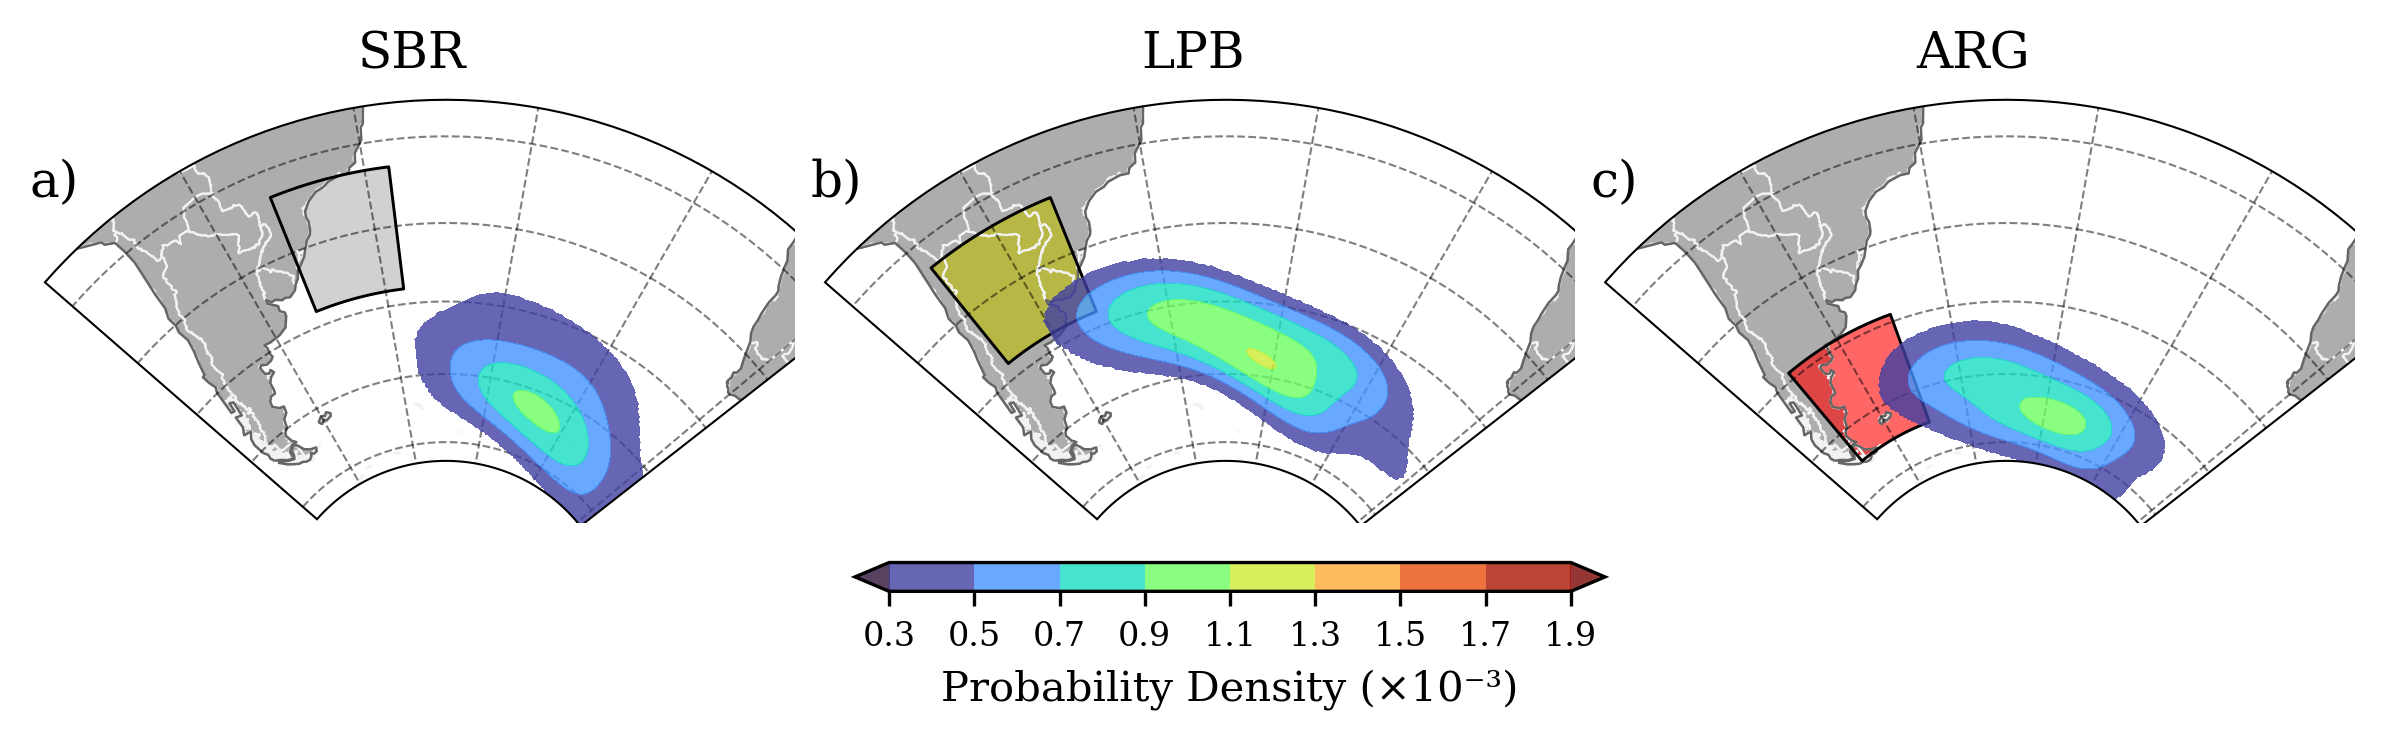
\includegraphics[width=\textwidth]{images/geral/vort_p90_vf.png}
\caption[Localização do mínimo de vorticidade (subconjunto p90)]{Semelhante à Figura~\ref{fig:loc_vort_global}, mas para o subconjunto p90 (sistemas mais intensos, decil inferior de $\zeta_{850}^{\min}$).}
\label{fig:loc_vort_p90}
\end{figure}

Sobre o subconjunto p90, comparando-o sistematicamente com a PG, aplica-se integralmente o fluxo metodológico descrito nas seções seguintes para avaliar se uma maior intensidade dinâmica do vórtice se associa a mudanças em: (i) a magnitude absoluta dos máximos de vento e precipitação; (ii) a distribuição espacial relativa desses máximos; e (iii) os padrões estruturais dominantes identificados pelo MEOF.

% ============================================================
%  SEÇÃO M3 — PROCESSAMENTO SEMILAGRANGEANO
% ============================================================

\section{Processamento semilagrangeano}\label{sec:procesamiento_lagrangiano}

Para caracterizar a estrutura dos sistemas independentemente de sua localização geográfica, adota-se o referencial semilagrangeano exposto na Seção~\ref{subsec:tb_lagrangiano} dos Fundamentos, um domínio móvel de $20^{\circ} \times 20^{\circ}$ centrado na posição do mínimo de vorticidade para cada instante $t$ da trajetória, em coordenadas relativas $(\Delta x, \Delta y)$ em relação ao núcleo ciclônico. Esse domínio isola o sinal de mesoescala e representa fisicamente a extensão espacial dos braços frontais do sistema, dimensão também usada por \citet{cardoso2022synoptic} no Atlântico Sul. O processamento é realizado separadamente para cada combinação de região de ciclogênese e fase do ciclo de vida.

Seguindo a técnica de compositing centrado no sistema (Seção~\ref{subsec:tb_compositing}), aplica-se uma média temporal centrada para reduzir a variabilidade de alta frequência dos dados horários e obter o campo mais representativo de cada fase. Para cada ciclone e fase, são promediados unicamente os registros horários mais próximos ao ponto médio temporal dessa fase: dois registros quando sua duração total é par (os dois passos centrais, equidistantes do ponto médio), e três quando é ímpar (o passo central exato mais um adjacente de cada lado). Esse critério evita que a média misture dois regimes evolutivos distintos, de modo que o campo resultante representa a condição arquetípica da fase (incipiente, intensificação, maturidade ou decaimento) e não uma transição entre estados sucessivos. O resultado é um único campo médio por combinação ciclone--fase, unidade de análise de todas as etapas estatísticas subsequentes. Consequentemente, cada ciclone contribui com exatamente um campo para cada uma das quatro populações fase-específicas de sua região, de modo que o tamanho amostral $m$ é constante entre fases dentro de uma mesma região e igual ao número de ciclones reportado na Tabela~\ref{tab:conteo_ciclones}.

% ============================================================
%  SEÇÃO M4 — CARACTERIZAÇÃO ESTATÍSTICA UNIVARIADA
% ============================================================

\section{Caracterização estatística univariada}\label{sec:tecnicas_estadisticas}

\subsection{Extração de máximos e distribuição de probabilidade (PDF)}\label{subsec:extraccion_pdf}

Sobre o campo médio por ciclone--fase aplica-se um suavizado espacial bidimensional com filtro gaussiano ($\sigma = 0.25$, biblioteca \texttt{scipy}) para evitar valores isolados em escala de ponto de grade. Em seguida, delimita-se a área de análise com uma máscara circular de $9.5^{\circ}$ de raio centrada no núcleo do sistema, inscrita no domínio de $20^{\circ} \times 20^{\circ}$ centrado no ciclone, de modo que uma faixa perimetral de $0.5^{\circ}$ em cada borda fica excluída. Dentro desse raio identificam-se: (i) a magnitude do valor máximo absoluto da variável de interesse, $x_i$, e (ii) sua localização em coordenadas relativas ao centro do ciclone, $\mathbf{s}_i = (\Delta x_i, \Delta y_i)$. O procedimento gera, para cada combinação de região, fase evolutiva e variável, um conjunto de $m$ pares magnitude--localização (um por evento ciclônico).

Para caracterizar a distribuição das magnitudes máximas extraídas $\{x_i\}_{i=1}^{m}$ estima-se a função de densidade de probabilidade (PDF) mediante KDE; sua justificativa em relação a histogramas e sua formulação matemática são apresentadas na Seção~\ref{subsec:tb_kde} dos Fundamentos. A implementação usa a classe \texttt{gaussian\_kde} de \texttt{scipy.stats}, com largura de banda $h$ segundo a regra de Scott (Equação~\ref{eq:scott_rule}) e o núcleo gaussiano (Equação~\ref{eq:tb_gaussian_kernel}) dos Fundamentos. As curvas PDF permitem contrastar quantitativamente como as magnitudes evoluem ao longo do ciclo de vida e como diferem entre a PG e p90.

\subsection{Distribuição espacial dos máximos}\label{subsec:kde_localizacion}

Para caracterizar a localização preferencial dos máximos em relação ao centro do ciclone, a posição relativa de cada máximo é tratada como variável aleatória bidimensional $\mathbf{S} = (\Delta x, \Delta y)$. A partir do conjunto de $m$ localizações relativas $\{\mathbf{s}_i\}_{i=1}^{m}$ da etapa anterior, estima-se a função de densidade de probabilidade da posição (PDFe), $\hat{f}(\mathbf{s})$, mediante o estimador kernel bidimensional da Seção~\ref{subsec:tb_kde} (Equações~\ref{eq:tb_kde_simple}--\ref{eq:tb_gauss_kernel_2d_simple}).

Diferentemente da PDF de magnitudes (Seção~\ref{subsec:extraccion_pdf}), a PDFe quantifica a densidade de probabilidade de que o máximo ocorra em uma posição relativa dada $\mathbf{s} = (\Delta x, \Delta y)$, independentemente do valor numérico de precipitação ou vento nesse ponto. O resultado é um campo contínuo de densidade de probabilidade sobre o domínio centrado.

\subsection{Análise de Funções Ortogonais Empíricas (EOF) univariada}\label{subsec:eof_univariado}

Para identificar os padrões espaciais dominantes de variabilidade estrutural, aplica-se uma análise EOF sobre o conjunto de $m$ campos médios por ciclone--fase, separadamente para cada variável (precipitação, vento), região e fase. As referências prévias desse enfoque foram apresentadas na Seção~\ref{subsec:tb_eof}. Antes da análise, subtrai-se de cada campo a média do conjunto em cada ponto de grade para obter as anomalias estruturais:

\begin{equation}\label{eq:eof_anomalia}
    X'(\tau, \mathbf{s}) = X(\tau, \mathbf{s}) - \frac{1}{m}\sum_{\tau'=1}^{m}X(\tau', \mathbf{s}),
\end{equation}

em que $X(\tau, \mathbf{s})$ é o campo da variável para o ciclone $\tau$ na posição relativa $\mathbf{s} = (x,y)$.

A análise EOF univariada se aplica em duas instâncias, com um tratamento ligeiramente distinto dessa anomalia segundo o propósito.

\paragraph{Modos dominantes e variância explicada.} Para as figuras de EOF1 e de fracionamento de variância (Seções~\ref{subsec:eof1_wind10_global}--\ref{subsec:eof1_wind10_p90}, \ref{subsec:eof1_tp_global}--\ref{subsec:eof1_tp_p90}, \ref{sec:var_exp_wind10} e \ref{subsec:var_exp_tp}), a anomalia é normalizada por um escalar global, com a mesma lógica aplicada ao MEOF (Seção~\ref{subsec:eof_multivariado}, Equação~\ref{eq:meof_normalizacion}):

\begin{equation}\label{eq:eof_normalizacion}
    Z(\tau, \mathbf{s}) = \frac{X'(\tau, \mathbf{s})}{\bar{\sigma}_X}, \qquad \bar{\sigma}_X = \frac{1}{N_s}\sum_{i=1}^{N_s} \sigma_X(\mathbf{s}_i),
\end{equation}

em que $\sigma_X(\mathbf{s}_i)$ é o desvio padrão entre ciclones no ponto de grade $\mathbf{s}_i$. Esse escalar único preserva a forma espacial da anomalia enquanto normaliza sua magnitude, e é calculado de forma independente para cada variável, região e fase mediante \texttt{scikit-learn}. Como consequência, as cargas de EOF$_k$ mostradas nos mapas são adimensionais (em unidades de $\bar\sigma_X$), não a magnitude física original da variável.

\paragraph{Significância estatística.} Para o teste Bootstrap-t (Seção~\ref{subsec:bootstrap_significancia}), o EOF é calculado diretamente sobre a anomalia $X'(\tau,\mathbf{s})$ sem essa etapa de normalização, mediante a biblioteca \texttt{xeofs} \citep{rieger2024xeofs} sobre estruturas \texttt{xarray}. Dado que ambos os procedimentos diferem unicamente por um fator de escala constante, igual para todo o domínio e todos os ciclones de um grupo, o percentual de variância explicada por cada modo é idêntico entre ambos; apenas muda a unidade das cargas espaciais, que nesse caso conservam a magnitude física original da variável.

Em ambos os casos, a reconstrução do campo a partir dos modos ortogonais segue a mesma expressão geral:

\begin{equation}\label{eq:eof_reconstruccion}
    X'(\tau, \mathbf{s}) = \sum_{k=1}^{K} \text{PC}_k(\tau) \cdot \text{EOF}_k(\mathbf{s}).
\end{equation}

Não se aplica remoção de tendência temporal (\textit{detrend}). O eixo amostral é um índice de eventos discretos com espaçamento temporal irregular entre 1979--2020, de modo que um ajuste linear cronológico assumiria erroneamente um espaçamento constante. O objetivo físico é isolar as características morfológicas da variabilidade inter-sistêmica dentro de cada fase, não as tendências climáticas de baixa frequência.

Cabe destacar que o tamanho amostral $m$ difere substancialmente entre regiões (Tabela~\ref{tab:conteo_ciclones}). ARG possui a amostra mais numerosa (1980 na PG, 198 em p90), enquanto SBR e LPB apresentam amostras consideravelmente menores (641/64 e 669/67, respectivamente). Essa assimetria implica que os autovetores de SBR e LPB estão sujeitos a maior incerteza de amostragem do que os de ARG, o que motiva a avaliação de significância estatística mediante Bootstrap-t descrita na Seção~\ref{subsec:bootstrap_significancia}.

A interpretação física de cada modo --como fluxo sinótico de fundo ou como circulação de mesoescala-- se apoia na escala espacial do padrão, sua localização relativa ao centro do ciclone e sua comparação qualitativa com a literatura; não se contrasta aqui com vento vetorial, diagnósticos frontais independentes ou índices de circulação de grande escala. Essas atribuições são lidas, portanto, como leituras fisicamente plausíveis, e não como identificações confirmadas.

\subsection{Significância espacial: Bootstrap-t}\label{subsec:bootstrap_significancia}

Para avaliar a robustez estatística dos autovetores do EOF e isolar os sinais físicos do ruído estocástico, implementa-se a reamostragem não paramétrica Bootstrap-t; sua escolha e vantagens em relação ao Bootstrap percentílico padrão para distribuições assimétricas e de cauda pesada foram fundamentadas na Seção~\ref{subsec:tb_bootstrap} dos Fundamentos. Geram-se $R = 15{,}000$ subamostras com reposição, garantindo erro de Monte Carlo insignificante na estimação das caudas da distribuição.

Para cada iteração $b$, recalcula-se o EOF sobre a subamostra e, em cada ponto de grade, calcula-se a estatística:

\begin{equation}\label{eq:bootstrap_t_espacial}
    t^*_b(\mathbf{s}) = \frac{\hat{\theta}^*_b(\mathbf{s}) - \hat{\theta}(\mathbf{s})}{SE^*_b(\mathbf{s})},
\end{equation}

em que $\hat{\theta}(\mathbf{s})$ é a carga espacial original em $\mathbf{s}$, $\hat{\theta}^*_b(\mathbf{s})$ sua estimativa na subamostra, $SE^*_b(\mathbf{s})$ o erro padrão dessa subamostra, e $SE(\mathbf{s})$ o erro padrão da carga original (calculado sobre a amostra completa, sem reamostrar). Os intervalos de confiança a 95\% são obtidos invertendo os quantis empíricos $q_{\alpha/2}$ e $q_{1-\alpha/2}$ da distribuição de $t^*$ (com $\alpha = 0.05$):

\begin{equation}\label{eq:bootstrap_ci_espacial}
    \left(\hat{\theta}(\mathbf{s}) - q_{1-\alpha/2}\,SE(\mathbf{s}),\; \hat{\theta}(\mathbf{s}) - q_{\alpha/2}\,SE(\mathbf{s})\right).
\end{equation}

Um ponto de grade é considerado estatisticamente significativo quando seu intervalo de confiança exclui o zero, o que equivale a rejeitar, no nível $\alpha = 0.05$ já definido, a hipótese nula de que a carga espacial nesse ponto não difere de zero por acaso de amostragem.

\subsection{Análise das Componentes Principais (PC1--PC3)}\label{subsec:analisis_pc}

Além da decomposição espacial, será usada a Componente Principal do primeiro modo (PC1), que representa a amplitude de cada ciclone sobre o padrão estrutural dominante; a interpretação dessas estatísticas foi estabelecida na Seção~\ref{subsec:tb_eof} dos Fundamentos.
Calculam-se, para a série de PC1 de cada variável, região e fase, a assimetria ($\gamma_1$):
\begin{equation}\label{eq:pc1_asimetria}
    \gamma_1 = \frac{1}{m} \sum_{\tau=1}^{m} \left(\frac{PC_{1,\tau} - \overline{PC_1}}{\sigma_{PC_1}}\right)^3,
\end{equation}
e a curtose ($\gamma_2$):
\begin{equation}\label{eq:pc1_curtosis}
    \gamma_2 = \frac{1}{m} \sum_{\tau=1}^{m} \left(\frac{PC_{1,\tau} - \overline{PC_1}}{\sigma_{PC_1}}\right)^4 - 3.
\end{equation}

Para conectar fisicamente a estrutura dos campos de superfície com a intensidade do sistema, avalia-se a correlação de Spearman entre a PC1, a PC2 e a PC3 de cada variável, e a vorticidade relativa a 850 hPa associada.
Esta última é obtida dos mesmos instantes centrais usados para construir os campos compostos (Seção~\ref{sec:procesamiento_lagrangiano}), tomando o de maior magnitude entre eles como representativo da intensidade do sistema nessa fase; não deve ser confundida com o $\zeta_{850}^{\min}$ de toda a vida do ciclone empregado na Seção~\ref{subsec:grupo_global} para a seleção do subconjunto p90.

O sinal da PC indica de forma reprodutível a que lado do padrão dominante cada ciclone recai.
Correlacionar a PC com sinal contra uma variável externa testa, então, se esse lado do padrão está associado à intensidade do sistema, além do quão marcada esteja a projeção.
Emprega-se Spearman para não assumir normalidade na distribuição das PC.
Sua interpretação físico-estatística, o vínculo entre o lado do padrão dominante em que recai um ciclone e sua intensidade dinâmica, foi estabelecida na Seção~\ref{subsec:tb_eof} dos Fundamentos.
Dado que o sinal de cada EOF é uma convenção independente e arbitrária entre decomposições distintas (Seção~\ref{subsec:tb_eof}), comparar o sinal dessa correlação entre regiões, fases ou populações não é informativo por si só; os capítulos de resultados reportam, por isso, o valor absoluto da correlação, e discutem sua magnitude e significância estatística em vez de seu sinal.

Para avaliar se os padrões dominantes de precipitação e vento variam conjuntamente, calcula-se a correlação de Spearman entre a PC1 de precipitação e a PC1 do vento, dentro de cada região e fase.
Valores próximos a $+1$ ou a $-1$ indicam que o lado do padrão dominante de um campo está sistematicamente associado ao lado do padrão dominante do outro; valores próximos a $0$ sugerem que ambos os padrões variam de forma independente entre si.
Pela mesma razão, o sinal dessa correlação cruzada só é interpretável se se verifica explicitamente, para a região e fase específicas, onde se localiza o núcleo de carga positiva de cada EOF1; fora desse contexto verificado, reporta-se o valor absoluto.

% ============================================================
%  SEÇÃO M5 — ANÁLISE MULTIVARIADA E PROTÓTIPOS
% ============================================================

\section{Análise multivariada e protótipos estruturais}\label{sec:meof_prototipos}

\subsection{EOF combinado (MEOF) precipitação--vento}\label{subsec:eof_multivariado}

Para identificar os padrões espaciais dominantes da estrutura combinada de precipitação e vento, realiza-se uma análise EOF combinada (MEOF). Diferentemente da análise univariada, o MEOF captura modos de variabilidade conjunta que refletem a organização morfológica típica dos campos de superfície associados à dinâmica ciclônica. Os fundamentos dessa técnica, incluindo a necessidade de normalizar variáveis com unidades físicas dispares e a lógica da concatenação espacial do vetor de estado, foram expostos na Seção~\ref{subsec:tb_eof} dos Fundamentos. Embora o MEOF seja habitual em estudos de eventos simultâneos, aqui se emprega exclusivamente como ferramenta de síntese estrutural, para isolar as configurações espaciais mais recorrentes dos campos de superfície. O procedimento consta de três passos:

\paragraph{Passo 1 — Anomalias.} Calcula-se o campo de anomalias de cada variável em relação à média do conjunto (PG ou p90) em cada ponto de grade.

\paragraph{Passo 2 — Normalização por desvio padrão espacialmente promediado.} Para preservar os gradientes espaciais nativos de cada campo, a normalização usa um escalar global por variável, em vez da padronização ponto a ponto da PCA sobre matriz de correlação:
\begin{equation}\label{eq:meof_normalizacion}
    Z_{V}(\tau, \mathbf{s}) =
        \frac{V'(\tau, \mathbf{s})}{\bar{\sigma}_{V}},
    \qquad
    \bar{\sigma}_{V} = \frac{1}{N_s} \sum_{i=1}^{N_s} \sigma_{V}(\mathbf{s}_i),
\end{equation}
em que $V'$ é o campo de anomalias, $\sigma_{V}(\mathbf{s}_i)$ o desvio padrão entre eventos no ponto de grade $\mathbf{s}_i$, e $N_s$ o número de pontos de grade do domínio. Esse escalar preserva os gradientes espaciais enquanto equilibra o peso de ambas as variáveis na matriz de covariância, evitando que o campo de maior variância domine a decomposição conjunta, problema documentado para variáveis de unidades dispares em \citet{wilks2019statistical_ch13}.

\paragraph{Passo 3 — Concatenação espacial.} Os campos normalizados são concatenados para formar o vetor de estado combinado:

\begin{equation}\label{eq:meof_vector}
    \mathbf{Y}(\tau) = \big[ Z_P(\tau),\; Z_W(\tau) \big].
\end{equation}

O EOF aplicado à matriz combinada $\mathbf{Y}(\tau)$ produz modos conjuntos que explicam a variância conjunta do sistema. O MEOF$_1$ produz simultaneamente um padrão espacial para precipitação ($\text{EOF}_{1,P}$) e outro para vento ($\text{EOF}_{1,W}$), ambos extraídos do mesmo modo dominante de covariabilidade conjunta.

Tanto a PG quanto o subconjunto p90 são processados de forma independente com esse mesmo procedimento, de modo que os padrões estruturais resultam exclusivamente de sua própria covariância interna.

\subsection{Construção dos protótipos estruturais}\label{subsec:prototipos}

Para cumprir o Objetivo Específico 4, desenvolve-se um procedimento de síntese visual que integra em um único painel, para cada combinação região-fase, quatro fontes de informação estatística derivadas das análises anteriores. Cada protótipo se compõe de quatro camadas superpostas em coordenadas relativas ao centro do ciclone $(\Delta x, \Delta y)$, dentro do domínio de $9.5^{\circ}$ de raio. A lógica do compositing centrado no sistema, que torna possível essa superposição, foi apresentada na Seção~\ref{subsec:tb_compositing} dos Fundamentos.

As duas primeiras camadas são as isolinhas da PDFe da localização de máximos de precipitação e vento. A partir da superfície de densidade $\hat{f}(\mathbf{s})$ (Equação~\ref{eq:tb_kde_simple}) extraem-se os contornos dos percentis 75 e 90 da densidade acumulada, e sobre cada superfície sinaliza-se com um marcador a coordenada $(\Delta x_{\text{moda}}, \Delta y_{\text{moda}})$, a posição onde é mais frequente encontrar o máximo da variável.

As camadas terceira e quarta mostram as isolinhas dos padrões espaciais do primeiro modo EOF univariado de cada campo ($\text{EOF}_{1,P}$ para precipitação e $\text{EOF}_{1,W}$ para vento), obtidos segundo a Seção~\ref{subsec:eof_univariado} e não do modo conjunto MEOF$_1$ (Seção~\ref{subsec:eof_multivariado}); essa escolha é justificada no Capítulo~\ref{cap:prototipos}.
Antes do traçado de contornos, aplica-se um suavizado gaussiano ($\sigma = 2$) a cada campo. Os níveis de contorno são determinados mediante percentis aplicados separadamente sobre os valores positivos (percentis 33 e 66, linha sólida) e negativos (percentis 33 e 66 do valor absoluto, linha descontínua).
Essa limiarização relativa garante comparabilidade entre diferentes combinações região--fase, independentemente da magnitude absoluta do padrão espacial do EOF.
As regiões de carga positiva indicam setores onde a variável tende a apresentar anomalias positivas em relação à média quando o modo dominante se ativa; as de carga negativa, supressão relativa.

O resultado se organiza em uma figura matricial de $3 \times 4$ painéis (3 regiões de ciclogênese $\times$ 4 fases evolutivas), em que cada painel integra as quatro camadas descritas: PDFe de precipitação, PDFe de vento, $\text{EOF}_{1,P}$ de precipitação e $\text{EOF}_{1,W}$ de vento.
A superposição permite ler o grau de organização espacial entre ambos os campos no entorno do ciclone: uma alta coincidência entre o núcleo do PDFe de precipitação e a região de carga positiva do EOF de vento indica uma estrutura frontal compacta; uma separação entre ambos revela assimetrias na distribuição dos máximos.
Essa análise caracteriza a morfologia da fase e, de forma secundária, oferece um referencial para identificar configurações que favoreceriam eventos simultâneos de vento e precipitação.

A coordenada de cada variável, anotada na legenda interna de cada painel como $(\Delta x, \Delta y)$ em graus, quantifica o deslocamento preferencial dos máximos em relação ao centro do vórtice.
Esse procedimento é executado de forma independente para a PG e o subconjunto p90, permitindo a comparação direta dos padrões estruturais entre ambos os estratos de intensidade.
